\section{Manifestations of \cpv, \cpv\ measurements}
\label{sec:CPVinB}
 In the SM, the CKM matrix is the only source of \cp\ violation. Therefore, all \cp\ violation measurements have to measure the phases of the CKM
 matrix. We remember from basic Quantum Mechanics that absolute phases
 cannot be measured, so what we need is phase differences. Phase
 differences show up in interference experiments (remember the double
 slit experiment - all what follows will in essence be that).

 \textbf{All CP violation measurements are interference experiments}
 where we have more than one path from an initial state to a final state, and the
 phase difference between the two (or more) paths shows up in the measured decay
 rates.
 
 \fbox{\parbox{0.9\textwidth}{\paragraph{Which CKM phases} If you want to figure out which CKM phases (e.g $\beta, \gamma$ or a combination like $2\beta -\gamma$) a certain decay is sensitive to, find out which decay diagrams could interfere and find out their CKM phases. If a \cpv\ parameter can be measured in this decay, it will be the phase difference between those two diagrams - even if you don't know at all how the measurement is done in practice}}
 
 In this section we will concentrate on \cpv\ in B hadrons. This is where \cpv\ effects are largest, and this is also where they can be connected best to specific CKM parameters.
 
\subsection{Types of \cp\ violation}

\subsubsection{CP violation in the mixing ("indirect CP violation")}
This is when the mass/width eigenstates do not match the CP eigenstates.
This is the dominant type of CP violation in the kaon system. This is expressed by the parameter $\epsilon$ in 
\begin{eqnarray}
\ket{\Kl} &=& \frac{1}{\sqrt{1 + \epsilon^2}} \left(
             \ket{K_{\mathsf{odd}}} + \epsilon \ket{K_{\mathrm{even}}} \right)
             \nonumber\\
\ket{\Ks} &=& \frac{1}{\sqrt{1 + \epsilon^2}} \left(
             \ket{K_{\mathsf{even}}} - \epsilon \ket{K_{\mathrm{odd}}} \right)
\end{eqnarray}
where $\epsilon$ is small, about $2.2\E{-3}$.
This is often also called "indirect \cpv". This type of \cpv\ is negligible in \Bdo\ and \Bso\ meson decays.

\paragraph{What interferes with what?}
$K^0 \to K^0$ with $K^0 \to \bar{K}^0 \to K^0$

(Sidenote: There is also direct \cpv\ in the kaon system, it's even smaller than indirect \cpv\ and it's measured by $\epsilon'$. This was historically very important, but we will not look into this parameter in this course, as there are much "cleaner" (easier to interpret in terms of CKM phases) direct \cp\ violation measurements in B meson decays.)

\paragraph{Indirect \cpv\ in the $B$ system}


In the $B$ system (($B^0$, or $B_s$) indirect \cpv\ is expected to be very small in the SM due to the CKM factors involved in the mixing. However sources beyond the SM can induce large indirect \cpv\ effects.
The typical way that experimentalists try to measure \cpv\ the $B$-system is through the ``flavour-specific" decays of $B^0\to D^-\mu^+\nu_{\mu}$ or  $B_s \to D_{s}^{-}\mu\nu_{\mu}$. These types of decays are called flavour specific because of the fact that for instance, the $B^0$ cannot decay to $D^+\mu^-\bar{\nu}_{\mu}$ but the $\bar{B}^0$ can (due to conservation of electric charge). This means that one can identify the whether the $B$-meson was a $B^0$ or a $\bar{B}^0$ when it decayed, simply by looking at the decay products. Another way of saying this, is that the amplitude 
\begin{equation}
\bra{B^{0}}\hat{H}_{W}\ket{D^+\mu^-\bar{\nu}_{\mu}} = \bra{\bar{B}^{0}}\hat{H}_{W}\ket{D^-\mu^+\nu_{\mu}} = 0
\end{equation}
where $\hat{H}_{W}$ is the weak Hamiltonian that mediates the decay.

As indirect \cpv\ would imply that the rate of $B\to\bar{B}$ is different compared to that of $\bar{B}\to B$, it is also important to know the flavour of the $B$ when it was produced. This is done by using a range of techniques (depending on the experiment). It is called flavour-tagging and the details of this method are beyond the scope of this course. 

Armed with the flavour of the $B$ at production and decay, experimentalists can measure the asymmetry $a_{sl}$ (``$sl$" for semileptonic owing to the final state of the $B$) given by
\begin{equation}
a_{sl}=\frac{\Gamma(\bar{B}^{0}\to B^0\to  D^-\mu^+\nu_{\mu}) - \Gamma(B^{0}\to \bar{B}^0\to  D^+\mu^-\bar{\nu}_{\mu})}{\Gamma(\bar{B}^{0}\to B^0\to  D^-\mu^+\nu_{\mu}) + \Gamma(B^{0}\to \bar{B}^0\to  D^+\mu^-\bar{\nu}_{\mu})} = \frac{1-|q/p|^4}{1+|q/p|^4}
\end{equation}
In the absence of indirect \cpv\, $a_{sl}=0$ and therefore $|q/p|=1$ as we discussed in Sec~\ref{sec:bosc}.


\subsubsection{CP violation in the decay ("direct \cpv")}
This is when the decay rates for some initial state $i$ to a final state $f$ are not the same as for the \cp--conjugate decay. For example
\[
\Gamma(\Bm \to (\Kp\pim)_D K^-) \neq \Gamma(\Bp \to (\Km\pip)_D K^+) 
\]
is a case of large direct \cpv\ discussed in detail further below.

In general, direct \cpv\ occours when two or more decay amplitude interfere. $A_i e^{\phi_i + \delta_i}$ with magnitude $A_i$,  CP-violating phases $\phi_i$ and CP-conserving phases (due to the strong interaction) $\delta_i$, rates for the process $B\to f$ described by the sum of these amplitudes are given by:
\begin{equation}
\Gamma(B \to f) \propto \left| A_1 e^{i\left(\phi_1 + \delta_1\right)} + 
|A_2 e^{i\left(\phi_2 + \delta_2\right)} \right|^2
= A_1^2 + A_2^2 + 2 A_1 A_2 
\cos(\Delta \delta + \Delta \phi)
\end{equation}
where $\Delta\delta = \delta_1 - \delta_2$ and $\Delta \phi = \phi_1 - \phi_2$. Under CP we find
\begin{equation}
\Gamma(\overline{B} \to \overline{f}) \propto \left| A_1 e^{i\left(-\phi_1 + \delta_1\right)} + 
|A_2 e^{i\left(-\phi_2 + \delta_2\right)} \right|^2
= A_1^2 + A_2^2 + 2 A_1 A_2 
\cos(\Delta \delta - \Delta \phi)
\end{equation}

A notable feature is that direct \cpv\ requires not only a phase difference in CKM phases, but also in the strong interaction.

\paragraph{What interferes with what?} 
$A_1 e^{\phi_1 + \delta_1}$ with $A_2 e^{\phi_2 + \delta_2}$, both amplitudes with the same initial and final state. For example:
$\Bm \to \Do \Km, \Do \to \Kp\pim$ with $\Bm \to \Dob \Km, \Dob \to \Kp\pim$


\subsubsection{CP violation in the interference between mixing and decay}
 The \emph{classic} \cp\ violation experiment in B physics makes use
 of the ``interference between decay and mixing''. At the basis of the
 measurement is B mixing, which allows a \Bdo\
 meson to change into a \Bdob\ meson. This works for other neutral
 meson systems, too, like \Bso\ mesons or neutral Kaons.

 Then need a decay that is accessible to both, \Bdo\ and \Bdob. A
 \cp\ eigenstate is a good pick. Let's call it $f_{CP}$. Now, if we
 have two decay paths to the same final state:
\begin{enumerate}
 \item \prt{\Bdo \to f_{CP}}
 \item \prt{\Bdo \to \Bdob \to f_{CP}}
\end{enumerate}
 The interference effects between the two path let us measure \cp\ violating phases.
\paragraph{What interferes with what?}
\prt{\Bdo \to f} with \prt{\Bdo \to \Bdob \to f}

\subsubsection{The \prt{\Bo \to \Bob} box diagrams}
 What phase do we measure with this? It is the phase difference
 between the two decay paths. So we need to establish what phase is
 picked up in the \prt{\Bdo \to \Bdob} transition, and add to that the
 phase difference between \prt{\Bdo \to f_{CP}} and \prt{\Bdob \to
 f_{CP}}. For the latter we'll have to pick a specific final state for
 $f_{CP}$. But we'll start with the \prt{\Bdo \to \Bdob} transition,
 that is the same in all measurements of this kind.

 For this we write down the Feynman diagram for the \prt{\Bdo \to
 \Bdob} transition:
\begin{equation}
\includegraphics[width=0.5\textwidth]{fig/C_P_CP/feyn_mix_bw.pdf}
\end{equation}
 This is the famous \textbf{Box Diagram} for B mixing.

 Let's go step by step through this diagram:
\begin{itemize}
 \item Time flows from left to right.
 \item Arrows pointing from right to left indicated
 anti-particles. This is an awkward notation - it means that the b
 quark line on top is in fact a $\bar{b}$. It stems from the fact
 that, because of \cpt\ invariance, \cp\ should be the same as \ts. So
 instead of writing down $\bar{b}$ we ``just'' invert the arrow of time.
 Note that some authors will draw all arrows going from left to write
 and a bar over the $b$. That's OK. And many will do both, write
 $\bar{b}$ and the arrows from right to left - that is technically
 wrong, but is intended to mean the same thing, and if you want, you can also use that system, I'm not going to be too fussy.
 \item Another piece of awkward notation: A \Bdo\ meson is made of
 $\bar{b}, d$ and a \Bdob\ meson of $b, \bar{d}$.
 \item And finally, this is a so-called loop diagram. The loop is the
 box. Inside loops, the usual constraints that the decaying particle
 must be heavier than the sum of the products don't apply. That's why
 the $d\to t$ transition is allowed - because the $t$ is inside a
 loop.
\end{itemize}

We recognise the above diagram as
one that describes a \prt{\Bdo \to \Bob} transition. To establish the
phase of this diagram
\begin{itemize}
 \item At each vertex, write down the appropriate CKM matrix
 element
 \item Multiply them together, or equivalently, if it's only the phase
 you're after, add up the phases.
 \item For the above diagram, the elements and their phases are (we
 only go to \order{\lambda^3} in the Wolfenstein parameterisation):
 \begin{itemize}
 \item $V_{td} \propto e^{-i\beta}$
 \item $V_{tb}^* \propto e^{-i 0}$
 \item $V_{td} \propto e^{-i\beta}$ (again)
 \item $V_{tb}^* \propto e^{-i 0}$ (again)
 \end{itemize}
 So the total phase of this diagram is $-2\beta$.
\end{itemize}

 There is another diagram, the equally famous other \textbf{Box
 Diagram} for B mixing that also contributes to B mixing:
\begin{equation}
\includegraphics[width=0.5\textwidth]{fig/C_P_CP/feyn_mix2_bw.pdf}
\end{equation}
 If you repeat the exercise above, you'll find that it has exactly
 the same phase, so adding the two diagrams together still has a phase
 of $-2\beta$.

As we discussed above, the top contribution completely dominates (and two tops completely dominate over one) so that we can neglect diagrams like these:
\begin{equation}
\includegraphics[width=0.3\textwidth]{fig/C_P_CP/feyn_mix_c.pdf}
\;\;
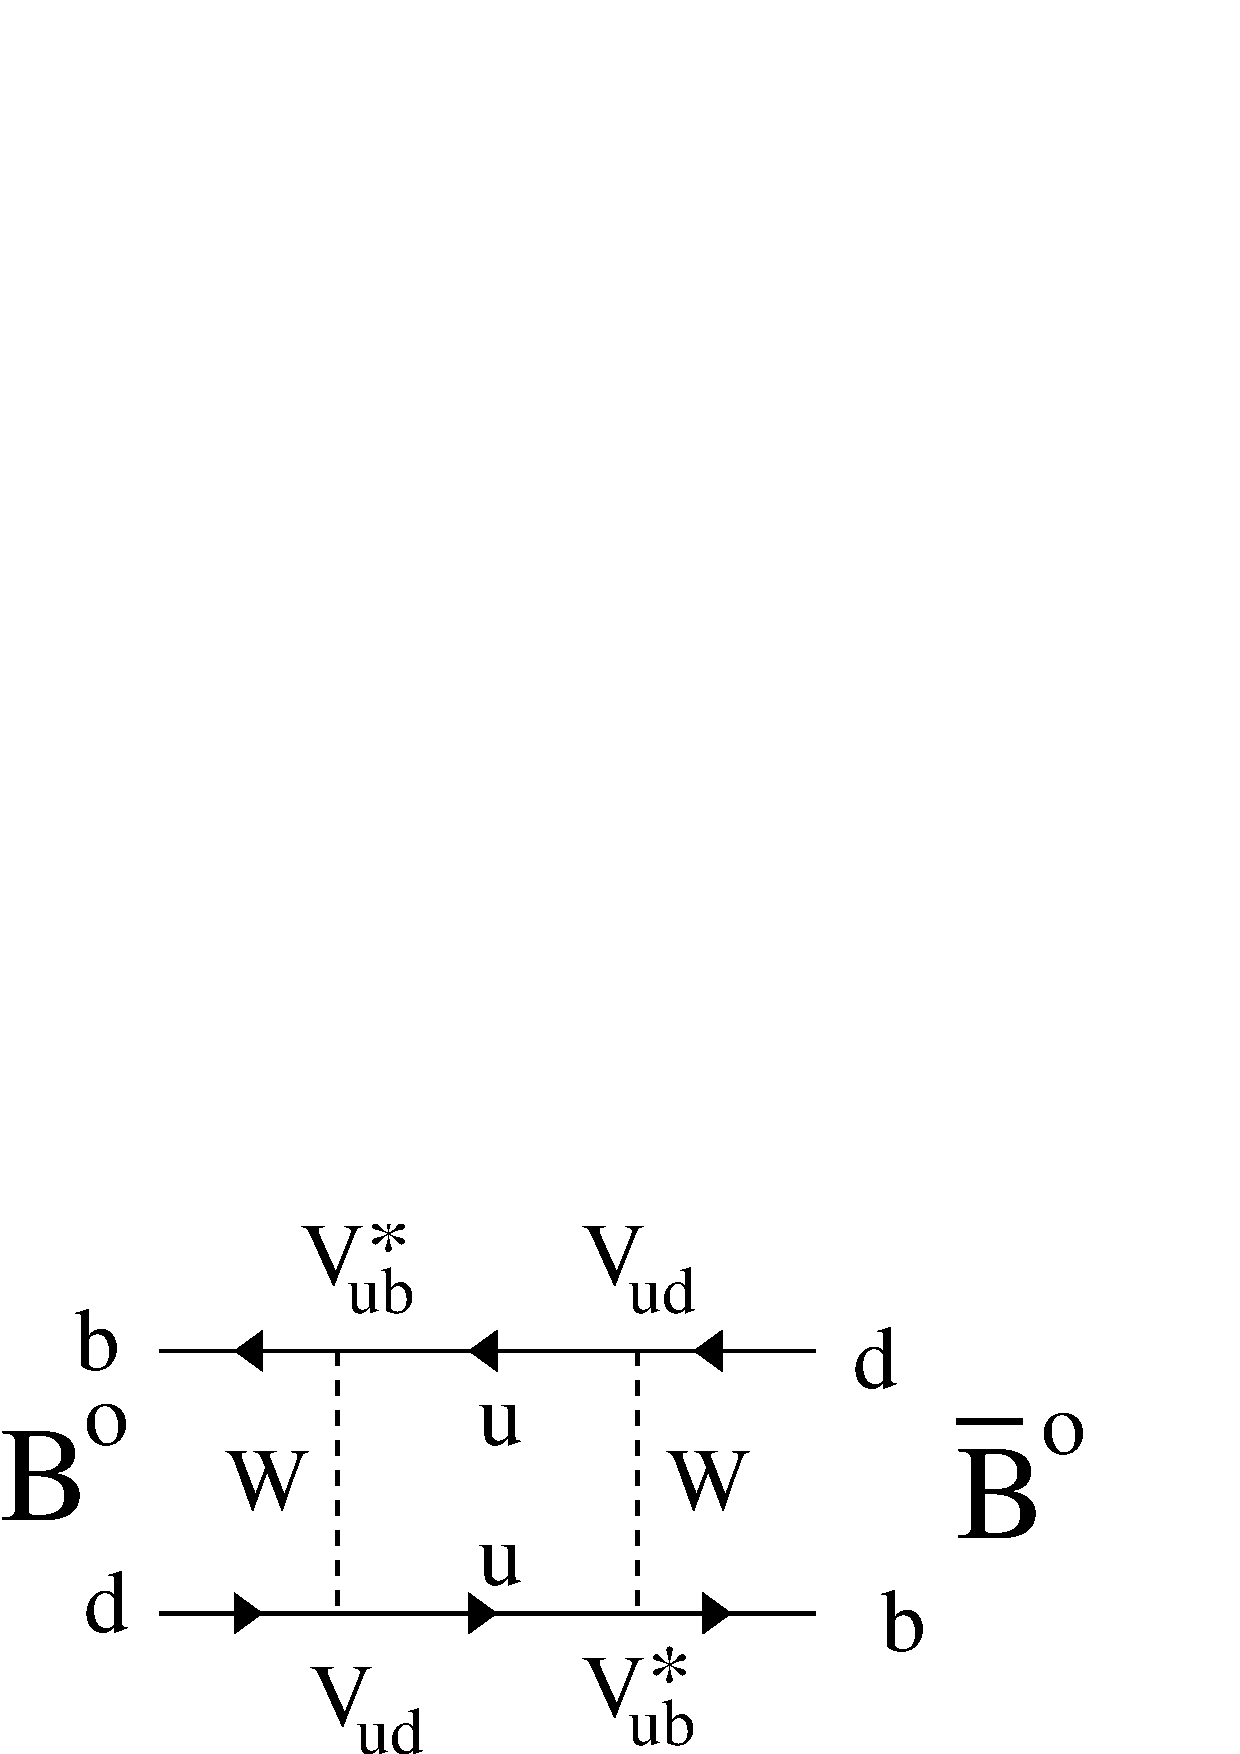
\includegraphics[width=0.3\textwidth]{fig/C_P_CP/feyn_mix_u.pdf}
\;\;
\includegraphics[width=0.3\textwidth]{fig/C_P_CP/feyn_mix_tu.pdf}
\end{equation}

\subsubsection{For example \prt{f_{CP} = K_s J/\psi}}

 The J/psi is a $c\bar{c}$ bound state - this is the particle that was
 actually seen when the charm quark was discovered. It has $J^{PC} =
 1^{--}$, it is a \cp\ even eigenstate. The $K_s$... well, because of
 \cp\ violation in the Kaon system, the $K_s$ is not a \cp\ eigenstate
 at all. But because \cp\ violation in the Kaon system is so much
 smaller than in the B system, for the purpose of this example, we
 can neglect this effect for now and assume that \Ks\ is \cp\ even. In real
 measurements, a correction for the small \cp\ violation in the Kaon
 system is applied, but it is really very small.

 So we have a CP-even eigenstate. But what does it contribute to the
 phase difference between
\begin{enumerate}
 \item \prt{\Bdo \to J/\psi K_s}
 \item \prt{\Bdo \to \Bdob \to J/\psi K_s}?
\end{enumerate}

 The tree-level (= no loops) diagram that contributes to this decay is:
\begin{equation}
 \includegraphics[width=0.5\textwidth]{fig/C_P_CP/feyn_btojpsiK_bw.pdf}
\end{equation}
 A few remarks about this one: The decay we drew is actually one with
 a $K^0$ in the final state - this has (neglecting \cp\ violation in
 the Kaon system) a 50\%- 50\% chance of decaying as a $K_s$ or a
 $K_L$. The way we know that it was a $K_s$ is that it decays within
 the detector volume. A $K_L$ would live too long to do that, and just
 escape.

 This diagram is proportional to $V^*_{cb} V_{cs}$, so (up to
 \order{\lambda^3}), it has phase $0$.
  
 The \cp-conjugate diagram, \prt{\Bob \to J/\psi K_s}, is 
\begin{equation}
 \includegraphics[width=0.5\textwidth]{fig/C_P_CP/feyn_bbbartojpsik.pdf}
\end{equation}
 This has also the phase $0$. We could have known that w/o writing
 down the diagram, of course - the weak phase of the \cp\ conjugate
 process is just the negative of the original process.

There is another contribution to this decay, the so-called penguin
diagram. This looks like so:
\begin{equation}
 \includegraphics[width=0.5\textwidth]{fig/C_P_CP/feyn_btojpsiK_penguin_bw.pdf}
\end{equation}
 This is a loop diagram, and again it is the top quark that
 dominates the loop, and there is no phase from the corresponding matrix elements $V_{tb}^* V_{ts}$. This is one of the the reasons why $J/\psi \phi$ is referred to as the "golden mode" for measuring $\beta$: Both penguin and tree contribution have the same, zero phase. (The other reason is that the $J/\psi$ can be experimentally very cleanly reconstructed in the decay mode $J/\psi \to \mu^+ \mu^-$).)
 
\subsubsection{The strong phase}
 We neglected up to now that each decay diagram also involves the
 strong interaction, which is responsible for binding the quarks
 together into the observable mesons. But since the strong interaction
 is \cp\ symmetric, there won't be a strong phase difference between
 the two \cp\ conjugate decays \prt{\Bo \to J/\psi K_s} and \prt{\Bob
 \to J/\psi K_s}. So the overall phase difference between the two is
 zero.
\subsubsection{Putting it all together}
 So, the overall phase difference between the decays
\begin{enumerate}
 \item \prt{\Bdo \to J/\psi K_s}
 \item \prt{\Bdo \to \Bdob \to J/\psi K_s}
\end{enumerate}
 is $-2\beta$ from the mixing diagram, and $0$ from the decay
 diagrams.\footnote{We did not look at any phases due to the strong interaction - these can affect the decay but they do not matter here. The strong interaction is \cp\ conserving, so any strong phase that would be the same in \prt{\Bo \to J/\psi K_S} and the \cp-conjugate process \prt{\Bob \to J/\psi K_S} (remember that \prt{J/\psi K_S} is a \cp\ eigenstate). So here, any strong phases cancel in the phase difference.}
 This can be visualised like this
\\
\includegraphics[width=0.5\textwidth]{fig/C_P_CP/B2JpsiKs_beta}
\\
 The fact that all contribution to the decay mode (both,
 tree and penguin) enter with the same phase, makes it \textbf{The
 golden mode} for measuring the CKM phase $\beta$.

 So we established now that the measurable quantity in \prt{\Bdo \to
 J/\psi K_S} decay is $-2\beta$. But how is it measured? It is measured in time dependent decay rate asymmetries:
\begin{equation}
\label{eq:timedepasy}
A\!\left(t\right) =
\frac{   \Gamma\left(\Bo \to f \right)(t)
        -\Gamma\left(\Bob \to f \right)(t)
    }{
         \Gamma\left(\Bo \to f \right)(t)
        +\Gamma\left(\Bob \to f \right)(t)
    }
\end{equation}
 Such ratios are experimentally favourable because acceptance effects
 etc cancel in the ratio.
 In decays to \cp\ eigenstates, $A(t)$ is given by
\begin{equation}
 A(t) = \mp \sin(\phi) \; \sin(\Delta\!m\, t)
\end{equation}
 where $\phi$ is the phase difference between the two decay paths, the one via mixing and the one without. For \prt{\Bdo \to
 J/\psi K_S}, $\phi = -2\beta$.
 
% \begin{figure}
% \includegraphics[width=0.5\textwidth]{fig/BELLE_B2JpsiKsAsy}
% \caption{Time-dependent decay rate asymmetry (\eqnref{eq:timedepasy}) in \prt{B^0 \to J/\psi K_S} (and related decays) as measured by the BELLE experiment in 2012. \href{https://inspirehep.net/record/1085529?ln=en}{Phys.Rev.Lett. 108 (2012) 171802}.\label{fig:tddra}}
% \end{figure}
 \begin{figure}
 \centering
 \includegraphics[width=0.6\textwidth]{fig/LHCb_B2JpsiKsAsy}
 \caption{Time-dependent decay rate asymmetry (\eqnref{eq:timedepasy}) in \prt{B^0 \to J/\psi K_S} (and related decays) as measured by the LHCb experiment in 2015 (\href{http://inspirehep.net/record/1355375/}{Phys.Rev.Lett. 115 (2015) no.3, 031601}). 
 The first (and still most precise) measurements of $\sin2\beta$ quantity are from BaBar
 and BELLE (both now stopped data taking, for their final results, see \href{https://inspirehep.net/record/812984?ln=en}{Phys.Rev. D79 (2009) 072009} \href{https://inspirehep.net/record/1085529?ln=en}{Phys.Rev.Lett. 108 (2012) 171802}). 
 The current world-average for $\sin(2\beta)$ from this type of measurement is $0.691 \pm 0.017$.
 The reason the amplitude in the plot is much smaller than $0.961$ is "mistag", mis-identification of \prt{B^0} and \prt{\overline{B}^0} at $t=0$. By knowing the probability for this to happen precisely, this can be corrected.
% corresponding to $\beta = 21.9^{\circ} \pm 0.7^{\circ}$ or $\beta = 68.1^{\circ}\pm 0.7^{\circ}$ (the other two values for $\beta$ compatible with $\sin(2\beta)=0.691\pm 0.017$ are excluded by  other measurements showing $\cos2\beta > 1$).
 For more results and averages, see \href{http://www.slac.stanford.edu/xorg/hfag/triangle/summer2016/index.shtml\#sin2b}{HFAG}.\label{fig:tddra}}
 \end{figure}
 \subsubsection{Summary of \cp\ violation in the interference between
 mixing and decay}
\label{sec:BCPSummary}

\begin{itemize}
 \item Mixing itself is not CP violating.
 \item By choosing the right decay mode, you can pick what you want to
 look at, \Bh, \Bl or \Bo, \Bob. Decays to flavour eigenstates see the
 \Bo, \Bob\ aspect and therefore the oscillation.
 \item Decays to \cp\ eigenstates would see \Bh\ and \Bl, if there were
 no CP violation - w/o CP violation no oscillation would be seen in
 such decays. The size of the oscillation that \emph{is} seen in decays to CP
 eigenstates measures \cp\ violation.
 \item The oscillation is best measured in ``time dependent decay rate
 asymmetries''. That is the number of \prt{\Bdo \to f} decay minus
 \prt{\Bdob \to f} decays divided by their sum, as a function of time,
 where \Bdo\ and \Bdob\ refers to the flavour at time
 $t=0$. Mathematically:
\begin{equation}
\label{eq:defasy}
A\!\left(t\right) =
\frac{   \Gamma\left(\Bo \to f \right)(t)
        -\Gamma\left(\Bob \to f \right)(t)
    }{
         \Gamma\left(\Bo \to f \right)(t)
        +\Gamma\left(\Bob \to f \right)(t)
    }
\end{equation}
 Such ratios are experimentally favourable because acceptance effects
 etc cancel in the ratio.
 \item In decays to \cp\ eigenstates, $A(t)$ is given by
\begin{equation}
 A(t) = \mp \sin(\phi) \; \sin(\Delta\!m\, t)
\end{equation}
 Where $\phi$ is the phase difference between the two interfering
 decay paths that we calculated above for the case of \prt{f=J/\psi
 K_s} where it is $-2\beta$.  The sign in front of $\sin(\phi)$
 depends on whether it is a CP-even or odd final state. For \cp\ even
 final states it's $-$, for \cp\ odd states it is $+$.
\item All of the above works for \Bdo\ as well as for \Bso\ (if you take
  into account the non-zero lifetime difference in \Bso\ system between \Bsl\
  and \Bsh, a few extra terms come into play - while these do
  matter for a precision measurement, we can ignore them for now).
\end{itemize}

To distill this even further:
\begin{itemize}
 \item \cp\ violation can be measured by measuring the
 \textbf{amplitudes of time dependent decay rate asymmetries}.
 \item For decays to \cp\ eigenstates \textbf{the amplitude of the
  asymmetry is the sine of the phase-difference between the
  interfering decay paths}.
\end{itemize}

 \subsection{Direct \cp\ violation (example question \& answers)}
\begin{enumerate}[a)]
\item Consider the decays \prt{B^- \to D^0 K^-} and \prt{B^- \to \overline{D}^0 K^-}. 
 \begin{itemize}
 \item Use the formula sheet to find out the quark content of the mesons involved.
 \answerbox{
 $\prt{B^-} = (b, \overline{u})$, \\
 $\prt{D^0} = (c, \overline{u})$ (and hence $\prt{\overline{D^0}} = (\overline{c}, u)$,\\
 $\prt{K^-} = (s, \overline{u})$.
 }
 \item Draw the tree-level Feynman diagrams that describe these decays. There are two topologies, they look like this:\\
 \begin{tabular}{cc}
 \includegraphics[width=0.3\textwidth]{problemsheets/ps2figs/CSup} &
 \includegraphics[width=0.3\textwidth]{problemsheets/ps2figs/CFav}
 \end{tabular}\\
 where the black blobs indicate that two quarks form a meson.
 \answerbox{The diagrams look like this:\\
\includegraphics[width=0.7\textwidth]{problemsheets/ps2figs/B2DKDiagrams.png}
}
 \item One of the topologies for the \prt{B^-} decay diagrams given above is "colour-suppressed". This means that the requirement that mesons are colourless objects restricts the colours that the quarks that result from this decay can have (while for the other diagram there is no such restriction). Which topology is colour suppressed? Explain, why.
 \answerbox{ (Remember, quarks can be red, green, blue, anti-quarks can
  be anti-red, anti-green, anti-blue; colourless objects can be made
  by combining three quarks: red + green + blue = white; or three
  anti-quarks: anti-red, plus anti-green plus anti-blue is also white;
  or by combining quark-antiquark pairs like red + anti-red, or green
  + anti-green, or blue + anti-blue.)
  \vspace{2ex}\\
  Topology (a) is colour suppressed. This is because in this diagram:
  \\\includegraphics[width=0.5\textwidth]{problemsheets/ps2figs/B2DK_supp}\\
  the \prt{B^-} is colour neutral, so it is a colour - anti-colour
  pair (say red and anti-red). The $\overline{c}$ and $s$ quark must
  then have the same anti-colour/colour as the $\overline{b}$ and $u$
  quark we started off with, in order to produce colour-less mesons
  (in our example anti-red, red). The \prt{B^-} is colourless, so if,
  for example, the $b$ is red, than the $\overline{u}$ must be anti-red }
 \item One of the two decays can proceed via both topologies (colour favoured and colour suppressed), the other only by one of them. To simplify the rest of the question a bit: for the decay where both topologies apply, only consider the colour favoured diagram and ignore the suppressed.
 \answerbox{... so this means that you should only consider these two diagrams:
 \\\includegraphics[width=0.4\textwidth]{problemsheets/ps2figs/B2DK_supp}, 
 \includegraphics[width=0.4\textwidth]{problemsheets/ps2figs/B2DK_fav}.
 }
 \item Estimate the complex value of the ratio of the two diagrams
  \[
    r_B e^{i\phi} = \frac{A(\prt{B^- \to \Dob K^-})}{\prt{A(B^- \to \Do K^-})}
 \]
 expressed as a magnitude $r_B$ and phase $\phi$. You obtain this value
 by multiplying together the vertex factors and multiplying the colour-suppressed diagram by $1/\sqrt{3}$ to take into account the colour suppression. 
 \end{itemize}
 \answerbox{
    The value of the \prt{\Bm \to \Dob \Km} diagram (i.e. the product of the relevant vertex factors) is $g_W V_{ub} \cdot g_W V^*_{cs}$. For \prt{\Bm \to \Dob \Km} it is $g_W V_{cb} \cdot g_W V_{us}^*$. The colour suppression introduces an additional factor of $1/\sqrt{3}$ to the \prt{\Bm \to \Dob \Km} diagram. So the ratio is:
    \[
    r_B e^{i\phi}  = \frac{A(\prt{B^- \to \Dob K^-})}{\prt{A(B^- \to \Do K^-})} = 
    \frac{V_{ub} \cdot V^*_{cs}}{\sqrt{3} \; V_{cb} \cdot V_{us}^*}
    \]
    From the formula sheet: 
    \begin{itemize}
     \item $V_{ub}   = 0.0037 \cdot e^{-i\gamma}$
     \item $V_{cs}^* = 0.97$
     \item $V_{cb}   = 0.041$
     \item $V_{us}^* = 0.23$
    \end{itemize}
    With this I get: $r_B e^{i\phi} = 0.22 e^{-i\gamma} = 0.22 e^{-i (68^{\circ})}$
 }
%%
\item Now consider the decay chains
\prt{B^- \to D^0 K^-, \Do \to K^+ K^-} and \prt{B^- \to \overline{D}^0 K^-, \Dob \to K^+ K^-}.
 \begin{itemize}
 \item Note that these two decay paths will interfere with each other - the situation is analogous to the double slit experiment:
 \\\includegraphics[width=0.5\textwidth]{problemsheets/ps2figs/B2DK_D2KK_interference}
 \item A bit of notation: To refer to the full decay that includes the interference between these decay paths, we write
 \prt{B^- \to (K^+ K^-)_D K^-}.
 Here, the notation \prt{(K^+K^-)_D} simply indicates that the \prt{K^+} and \prt{K^-} result from the decay of the \Do\ or \Dob. 
 \item Interference leads to sensitivity to phases - specifically, to sensitivity to the phase difference between the two decay paths. Your Feynman diagrams should indicate a phase difference of $\phi = -\gamma$ due to the weak interaction. This, however, neglects the effects of the strong interaction. This is difficult to calculate but it also leads to a phase difference, which we call $\delta_B$. So the total phase difference is $\phi = \delta_B - \gamma$.
 \item For the next step, it's useful to define:
 \begin{itemize}
 \item $C$ is the amplitude $A(\prt{B^- \to D^0 K^-})$.
 \item We write the amplitude ratio of \prt{B^- \to \Dob K^-} and \prt{B^- \to \Do K^-} as
 \[
    \frac{A(\prt{B^- \to \Dob K^-})}{\prt{A(B^- \to \Do K^-})} = r_B e^{i(\delta_B - \gamma)}
 \]  
 where $r_B$ is the magnitude of this ratio, $\delta_B$ the phase difference induced by the strong interaction, and $\gamma$ the CP violating one induced by the weak interaction.
 \item $K$ is the amplitude $A(\prt{ \Do \to K^+ K^-})$, which is the same as $A(\prt{ \Dob \to K^+ K^-})$ (you can check by drawing the diagrams and applying CKM factors).
 \end{itemize}
 With this, we can label our interference sketch with the relevant amplitudes like this:\\
 \includegraphics[width=0.5\textwidth]{problemsheets/ps2figs/B2DK_D2KK_interference_labelled}\\
 (This has no purpose other than visualising and organising what goes on, which can be helpful in the subsequent calculations.)
 \item If you apply the \cp\ operation to this amplitude ratio, you get:
  \[
    \frac{A(\prt{B^+ \to \Do K^+})}{\prt{A(B^+ \to \Dob K^+})} = r_B e^{i(\delta_B + \gamma)}
 \]
 Explain why.
 \answerbox{The strong interaction respects \cp\ symmetry, so all factors introduced by it (including the phase $\delta_B$) remain invariant. For the weak interaction, the \cp\ operation has the effect of complex conjugating the CKM matrix element, so we take the negative of all phases introduced by the CKM matrix, here: $\gamma \to -\gamma$. The magnitudes remain the same, so:
 $
 \left|\frac{A(\prt{B^- \to \Dob K^-})}{\prt{A(B^- \to \Do K^-})} \right| = 
 \left|\frac{A(\prt{B^+ \to \Do K^+})}{\prt{A(B^+ \to \Dob K^+})} \right|
 $
 and hence, the effect of \cp\ is: $r_B \to r_B$, $\delta_B \to \delta_B$, $\gamma \to -\gamma$.
 }
 \item Calculate the rate asymmetry
 \[
  A = \frac{ 
    \Gamma(B^- \to (K^+ K^-)_D K^-) -
    \Gamma(B^+ \to (K^+ K^-)_D K^+)
  }{ 
    \Gamma(B^- \to (K^+ K^-)_D K^-) +
    \Gamma(B^+ \to (K^+ K^-)_D K^+)
  }
 \]
 in terms of $r_B$, $\delta_B$, $\gamma$ (the $C$ and $K$ will cancel, if you want you can simply set them to $1$ straight from the beginning).
 \end{itemize}
 \answerbox{
     \begin{eqnarray*}
      \Gamma(B^-) & = & 
      \left| CK + CK r_B e^{i(-\gamma + \delta_B)} \right|^2
      \\ & = &
      C^2 K^2 \left(1 + r_B^2 + 2\,r_B\,\cos\left(-\gamma +\delta_B \right)\right)
      \\ & = & C^2K^2\left(1 + r_B^2 + 2\,r_B\, \left(
        \cos(\delta_B)\,\cos\gamma {\color{red} +} 
        \sin(\delta_B)\,\sin\gamma\right)\right)
      \\ \Gamma(B^+) & = & 
      \left| CK + CK r_B e^{i(+\gamma + \delta_B)} \right|^2
      \\ & = &
      C^2 K^2 \left(1 + r_B^2 + 2 r_B\,\cos\left(+\gamma +\delta_B \right)\right)
      \\ & = & C^2 K^2 \left(1 + r_B^2 + 2 r_B\, \left(
        \cos(\delta_B)\,\cos\gamma {\color{red} -}
          \sin(\delta_B)\,\sin\gamma\right)\right)
      \\ A_{CP}^{KK} & = & 
      \frac{
        2 r_B\,\sin(\delta_B)\,\sin\gamma
      }{
        1 + r_B^2 + r_B\, \cos(\delta_B)\,\cos\gamma
      } 
    \end{eqnarray*}
    }   
    \item Repeat the calculation for
  \[
  A = \frac{ 
    \Gamma(B^- \to (K^+ \pi^-)_D K^-) -
    \Gamma(B^+ \to (K^- \pi^+)_D K^+)
  }{ 
    \Gamma(B^- \to (K^+ \pi^-)_D K^-) +
    \Gamma(B^+ \to (K^- \pi^+)_D K^+)
  }
 \]
 Note that there will additional parameters because the ratio of the \Do, \Dob\ decay amplitudes does not cancel as in the case above, but instead:
  \[
    \frac{A(\prt{\Do \to K^+ \pi^-})}{A(\prt{\Dob\to K^+\pi^-})} = r_D^{K\pi} e^{i\delta_D}
 \]
 \answerbox{
    In the previous part, with used
    $\frac{A(\prt{\Do \to K^+ K-})}{A(\prt{\Dob\to K^+K-})}=1$, which is fundamentally because there is no \cp\ violation in \Do\ decays, and the final state is a \cp\ eigenstate. We could also have arrived at this result by drawing the Feynman diagrams for both decays, using the appropriate CKM matrix elements (and that the CKM matrix elements involved in \Do\ decays are all real is ultimately the reason that there is no \cpv\ in \Do\ decays).
     
    Now that the \Do, \Dob\ do not decay to a \cp\ eigenstate anymore we actually need to take into account that 
    \[
    \frac{A(\prt{\Do \to K^+ \pi^-})}{A(\prt{\Dob\to K^+\pi^-})} = r_D^{K\pi}  e^{i\delta_D}
    \]
    Note that there is no weak phase that would change under \cp. You can get this by drawing diagrams, or just remember that there is no \cpv\ in D meson decays. So $\delta_D$ is the strong phase difference between the \Do\ and \Dob\ decay amplitude to $\Kp\pim$.
    
    Our interference sketch looks now like this:
    \\\includegraphics[width=0.5\textwidth]{problemsheets/ps2figs/B2DK_D2Kpi_Interference}\\
    
     \begin{eqnarray*}
      \Gamma(B^-) & = & 
      \left| CK r_D^{K\pi} e^{i\delta_D^{K\pi}} + CK r_B e^{i(-\gamma + \delta_B)} \right|^2
      \\ & = &
      C^2 K^2 \left({r_D^{K\pi}}^2 + r_B^2 + 2r_D^{K\pi}\,r_B\,\cos\left(-\gamma +\delta_B-\delta_D^{K\pi} \right)\right)
      \\ & = & C^2K^2\left({r_D^{K\pi}}^2 + r_B^2 + 2r_D^{K\pi}\,r_B\, \left(
        \cos(\delta_B-\delta_D^{K\pi})\,\cos\gamma {\color{red} +}
        \sin(\delta_B-\delta_D^{K\pi})\,\sin\gamma\right)\right)
      \\ \Gamma(B^+) & = & 
      \left| CK r_D^{K\pi} e^{i\delta_D^{K\pi}} + CK r_B e^{i(+\gamma + \delta_B)} \right|^2
      \\ & = &
      C^2 K^2 \left({r_D^{K\pi}}^2 + r_B^2 + 2r_D^{K\pi}\,r_B\,\cos\left(+\gamma +\delta_B-\delta_D^{K\pi} \right)\right)
      \\ & = & C^2 K^2 \left({r_D^{K\pi}}^2 + r_B^2 + 2r_D^{K\pi}\,r_B\, \left(
        \cos(\delta_B -\delta_D^{K\pi})\,\cos\gamma 
        {\color{red} -} \sin(\delta_B-\delta_D^{K\pi})\,\sin\gamma\right)\right)
      \\ A_{CP}^{K\pi} & = & 
      \frac{
        2r_D^{K\pi}\,r_B\,\sin(\delta_B-\delta_D^{K\pi})\,\sin\gamma
      }{
        {r_D^{K\pi}}^2 + r_B^2 + 2r_D^{K\pi}\,r_B\, \cos(\delta_B-\delta_D^{K\pi})\,\cos\gamma
      } 
      \\ & = & 
      \frac{
        2\,\frac{r_B}{r_D^{K\pi}}\,\sin(\delta_B-\delta_D^{K\pi})\,\sin\gamma
      }{
        1 + \left(\frac{r_B}{r_D^{K\pi}}\right)^2 
        + 2\frac{r_B}{r_D^{K\pi}} \cos(\delta_B-\delta_D^{K\pi})\,\cos\gamma
      } 
      \\ & & \mbox{which is the same as}
        \\ & = & 
      \frac{
        2\,\frac{r_D^{K\pi}}{r_B}\,\sin(\delta_B-\delta_D^{K\pi})\,\sin\gamma
      }{
        1 + \left(\frac{r_D^{K\pi}}{r_B}\right)^2 
        + 2\frac{r_D^{K\pi}}{r_B} \cos(\delta_B-\delta_D^{K\pi})\,\cos\gamma
      } 
    \end{eqnarray*}
 }
 \item Which of the two asymmetries is larger? Estimate an approximate numerical value.
 \answerbox{The difference between the two asymmetries is that, to get from $A_{CP}^{KK}$ to $A_{CP}^{K\pi}$,  we need to replace $r_B$ with $r_B/r_D^{K\pi}$, or, equivalently with $r_D^{K\pi}/r_B$. The best sensitivity is reached for when this factor is $\sim 1$, to the question comes down to whether $r_B$ or $r_D^{K\pi}/r_B$ is closer to $1$ (note
 
 So let's estimate $r_D$. The relevant Feynman diagrams are:
 \\\includegraphics[width=0.65\textwidth]{problemsheets/ps2figs/D2KpiDiagrams}.\\
 Multiplying the relevant CKM matrix elements:
    \[
     \frac{A(\prt{\Do \to K^+ \pi^-})}{A(\prt{\Dob\to K^+\pi^-})}
     =
     \frac{V_{cd}^* V_{us}}{ V_{ud}^* V_{cs}}
     \approx \cos^2(\theta_C) = 0.05
    \]
 So, we estimate $r_D/r_B \sim 0.25$. It turns out that the measured values for $r_B$ is $0.01$, somewhat smaller than our estimate, while our estimate for $r_D$ is spot-on, so really, $r_D/r_B \sim 0.5$.
 
 To estimate the size of the asymmetry, we need to know $\delta_B$ and $\delta_D$. We cannot calculate those, but we can get an estimate of the maximum value that the asymetries can obtain by assuming they are such that the cosine of the strong phase differences is $0$ and the sine is $1$, leading to
 \begin{eqnarray*}
     A_{CP}^{KK} 
       & \leq & 
      \frac{
        2\,r_B\,\sin\gamma
      }{
        1 + r_B^2 
      }
  \\ A_{CP}^{K\pi} 
       & \leq & 
      \frac{
        2\,\frac{r_D^{K\pi}}{r_B}\,\sin\gamma
      }{
        1 + \left(\frac{r_D^{K\pi}}{r_B}\right)^2 
      } 
  \end{eqnarray*}
 Putting in the values we calculated in this exercise, we get
  \begin{eqnarray*}
     A_{CP}^{KK} 
       & \leq & 
      \frac{
        2 \cdot 0.22 \sin(68^{\circ})
      }{
        1 + 0.22^2 
      } = 0.38
  \\ A_{CP}^{K\pi} 
       & \leq & 
      \frac{
        2\cdot 0.25\,\sin(68^{\circ})
      }{
        1 + 0.25^2 
      } =0.48
  \end{eqnarray*}
 These are both quite large numbers (\cp\ assymetries of about 40-50\%, that's a big effect). Using the measured value of $r_B$ instead, we get
  \begin{eqnarray*}
     A_{CP}^{KK} 
       & \leq & 
      \frac{
        2 \cdot 0.1 \sin(68^{\circ})
      }{
        1 + 0.1^2 
      } = 0.18
  \\ A_{CP}^{K\pi} 
       & \leq & 
      \frac{
        2\cdot 0.5\,\sin(68^{\circ})
      }{
        1 + 0.5^2 
      } =0.74
  \end{eqnarray*}
 Now the difference between the two methods becomes much clearer. While $A_{CP}^{KK}$ can go up to $18\%$, $A_{CP}^{K\pi}$ could be as large as $74\%$!! \cp\ violation in the B hadrons is indeed not a small effect.
 }
\end{enumerate}

 

\subsection{Summary of \cpv\ phenomenology}
\begin{itemize}
\item There are three types of \cpv: \cpv\ in mixing, \cpv\ in decay, and \cpv\ in the interference between mixing and decay.
\item \cpv\ in mixing is the dominant \cp--violating effect in the Kaon system, while in the B system, it is negligible. The mechanisms of \cpv\ in B hadrons is direct \cpv\ and \cpv\ in the interference between mixing and decay.
\item \cpv\ is an interference effect, and needs therefore at least two interfering decay amplitudes.
\item \cpv\ can be very large in B-hadron decays, because it will involve, even at tree-level, all three generations (while in kaon decays, the 3rd generation only enters indirectly through loops). B hadrons give us access to the ony two CKM matrix element with large complex phases, $V_{td}$ (which enters in \Bdo\ mixing, usually measured time-dependent decay rate asymmetries) and $V_{ub}$ (in all decays involving $b \to u$ transitions).
\item We learnt how to calculate \cp-violating asymmetries in decays such as \prt{\Bm \to (K^+\pi^-)_D\Km} and its \cp-conjugate, and in \prt{\Bm \to (K^+K^-)_D\Km} and its \cp-conjugate.
\item We learnt how to calculate the amplitude of time-dependent decay rate asymmetries in \cp\ violation measurements in neutral B meson decays to \cp\ eigenstates like \prt{\Bdo \to J/\psi K_S}. It's the sine of the phase difference of the interfering decay paths.
\end{itemize}

